\documentclass{article}

\usepackage[utf8]{inputenc}
\usepackage[T1]{fontenc}
\usepackage{lipsum}
\usepackage{graphicx}
\usepackage{amsmath}
\usepackage[margin=1in]{geometry}
\usepackage{titlesec}
\usepackage{enumitem}

\titleformat{\section}
{\LARGE\bfseries}{\thesection}{1em}{}

\titleformat{\subsection}
{\Large\bfseries}{\thesection}{1em}{}

\begin{document}
\pagestyle{empty}
\section*{Design Pattern 4}
\large

\subsection*{Introduzione}
\large
Obiettivi:
\begin{itemize}
    \renewcommand{\labelitemi}{-}
    \itemsep0em
    \item Applicare propriamente i pattern del modello GoF 
\end{itemize}
Questa sezione rappresenta il naturale conseguimento del documento \textit{Design Pattern 3}, in cui sono elencati ulteriori pattern \textit{comportamentali}, \textit{creazionali} e \textit{strutturali} del \textit{catologo GoF}.

\subsection*{Memento (Behavioral Pattern)}
\large
\textit{Problema}\\
Come ripristinare un oggetto al suo stato precedente?\vspace*{14pt}\\
\textit{Soluzione}\\
Catturare ed esternalizzare lo stato interno dell'oggetto in maniera tale che possa essere restituito e ripristinato successivamente.\vspace*{14pt}\\
\textit{Memento} promuove l'utilizzo e l'implementazione di azioni di \textit{rollback}, le quali permettono il ripristino di un sistema oppure di un'istanza di classi allo stato precedente a \textit{modifiche}.\vspace*{7pt}\\
In relazione ad un \textit{pattern comportamentale} simile, è progettata un'entità software dedita esclusivamente alla memorizzazione dello \textit{snapshot} creato, la quale non deve sviluppare alcuna logica algoritmica differente; si ricordino i principi del modello \textit{GRASP}, in particolare \textit{high cohesion}, in cui classi software devono mantenere una \textit{coesione funzionale} al loro interno, ossia i metodi sviluppati devono garantire la modellazione di un unico comportamento, affinchè sia concrettizzata una soluzione di \textit{elevata qualità}. Il termine che si occupa di garantire un approccio simile è definito \textit{Memento}.\vspace*{7pt}\\
Pur di evitare incompresioni si attuano definizioni dell'entità coinvolte, in cui si osserva:
\begin{itemize}[label={-}]
    \itemsep0em
    \item \textit{Originator}, colei che pone e richiede la salvaguardia, all'interno di strutture dati apposite, del proprio stato, affinchè sia ripristinabile 
    \item \textit{Caretaker}, entità affine al \textit{domain layer}, la quale pone la ragione e l'arco temporale in cui il \textit{Originator} debba memorizzare e ripristinare il proprio stato. Per cui riassumendo raffigura il mandante dell'azione di ripristino
    \item \textit{Memento}, classe software progettata univocamente per la memorizzazione della \textit{rappresentazione opaca} dello stato, in modo tale che sia incomprensibile per \textit{high level classes} ed entità software, al di fuori di \textit{Originator} 
\end{itemize}
Un approccio come quello descritto è attuato per azioni di \textit{serializzazione}, ossia si tenta di rappresentare \textit{stati} di un oggetto attraverso una combinazione di byte, pur di adeguare operazioni di \textit{storage} all'interno di strutture dati persistenti. Infatti, in assenza di \textit{Memento}, sarebbe piuttosto complicato realizzare un \textit{vincolo comportamentale} come quello precedente, poichè non sarebbe possibile adeguare la traduzione in \textit{formato binario}, dato che linguaggi di programmazione legati al paradigma degli oggetti sostengono il principio di \textit{incapsulamento}, secondo cui gli attributi debbano essere privati oppure protetti all'interno di ogni singola classe, causandone la violazione.

\subsection*{Iterator (Behavioral Pattern)}
\large
\textit{Problema}\\
Come astrarre algoritmi che permettano l'accesso a strutture dati indipendentemente dalla collezione analizzata?\vspace*{14pt}\\
\textit{Soluzione}\\
Provvedere un modo per accedere sequenzialmente agli elementi di una collezione in modo tale che la sua rappresentazione non sia vincolante per l'iteratore.\vspace*{14pt}\\
L'idea pone che alla classe \textit{Iterator} sia assegnata la responsabilità di accedere e attraversare l'oggetto aggregato fornendo un protocollo comportamentale standard, a cui è applicata una strategia di \textit{astrazione} che provvede alla separazione della nozione di algoritmo dal concetto di struttura dati. 
La motivazione consiste nell'intento di garantire una tipologia di programmazione affine al paradigma orientato agli oggetti, riducendo in questa maniera l'ammontare di configurazioni e implementazioni singole per ogni struttura dati.\vspace*{7pt}\\
A titolo semplificativo è attuato un \textit{approccio} che possa favorire l'utilizzo di \textit{algoritmi} indipendentemente dalla \textit{struttura dati}, dove un atteggiamento differente richiederebbe un esteso range di \textit{permutazioni} da sviluppare e mantenere.\vspace*{14pt}\\
\textit{Caso di studio}\\
\begin{center}
    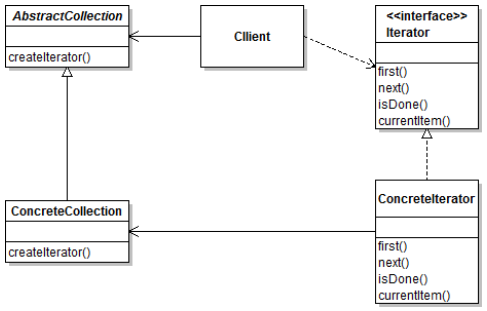
\includegraphics[width=0.5\textwidth]{foto 1.png}
\end{center}
Si analizzano le entità che rappresentano la raffigurazione, in cui:
\begin{itemize}[label={-}]
    \itemsep0em
    \item \textit{Client}, \textit{high level class} utilizzata da utenti finali, affine al domain model
    \item \textit{AbstractCollection}, al suo interno è mantenuto lo schema principale dell'algoritmo affinchè sottoclassi possano implementare step mancanti a seconda delle proprie specifiche, si osservi che un approccio del genere è stabilito dal \textit{behavioral pattern} \textit{template method}
    \item \textit{ConcreteCollection}, \textit{sottoclasse} derivata dalla \textit{superclasse} \textit{AbstractCollection}, la quale eredita attributi e metodi su cui sarà certamente adeguato \textit{polimorfismo}. Al suo interno è posta la responsabilità \textit{createIterator()}, ossia una \textit{doing resposability} che consenta la creazione e l'utilizzo di un'istanza della classe \textit{Iterator}
    \item \textit{InterfaceIterator}, \textit{interfaccia} applicata per soddisfare i principi di qualità del software del modello \textit{SOLID}, soprattutto in relazione al \textit{dipendency inversion principle} in cui classi legate alla logica algoritmica non debbano dipendere da entità affini al mondo reale; rispetto all'esempio, sarà mantenuta un'istanza del layer astratto all'interno del termine \textit{Client}, affinchè possa usufruire di metodi di \textit{accesso} e di \textit{attraversamento} della \textit{collezione} di oggetti mediante l'\textit{iteratore} 
    \item \textit{ConcreteIterator}, entità software che estende le funzionalità dell'\textit{interfaccia}, in modo tale che siano garantiti comportamenti interpellabili da collezioni di oggetti indipendentemente dalla \textit{struttura dati }
\end{itemize}

\subsection*{Visitor}
\large
\textit{Problema}\\
Come sviluppare un'applicazione comune a tutti gli elementi di una collezione, qualora all'interno della struttura dati di riferimento siano memorizzati oggetti eterogenei fra loro?\vspace*{14pt}\\
\textit{Soluzione}\\
Attuare una duplice gerarchia affinchè possano essere imbastiti flussi di controllo indipendentemente dalla tipologia di oggetto riscontrato.\vspace*{14pt}\\
Una prima risoluzione potrebbe essere garantita tramite l'impiego di un \textit{Iterator}, il quale garantisce l'accesso e l'attraversamento degli oggetti aggregati a cui poi sarà possibile attuare funzionalità desiderate; oppure automatizzare l'approccio mediante \textit{Visitor}.
La volontà di adeguare un pattern comportamentale simile avviene qualora si tenti di aumentare il numero di funzionalità, senza modificare classi concrete riferite agli \textit{Elementi} su cui opera il sistema software.\vspace*{14pt}\\
\textit{Caso di studio}\\
\begin{center}
    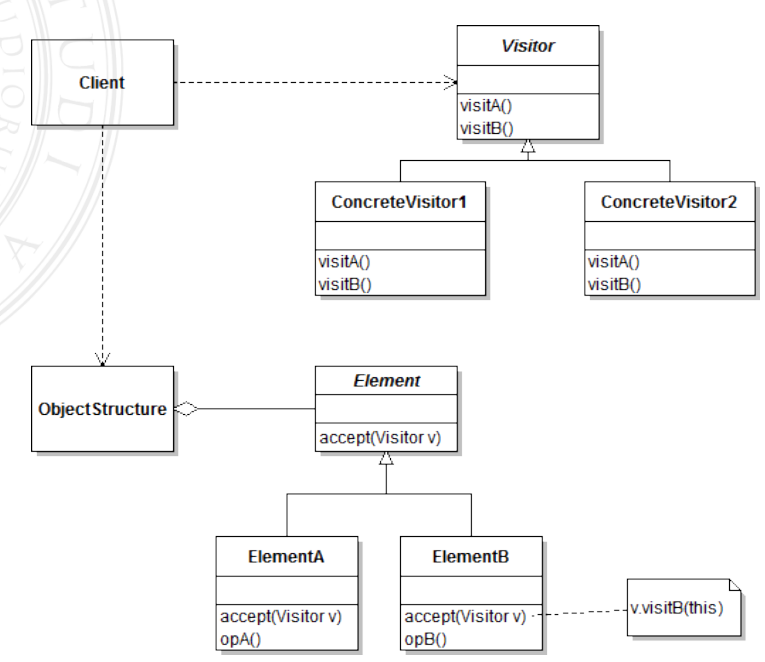
\includegraphics[width=0.65\textwidth]{foto 2.png}
\end{center}
Prima di addentrare la raffigurazione su specifiche comportamentali degli elementi che contraddistinguono il modello, si narrano due espressioni fondamentali per concepire al meglio l'intento del pattern, ossia:
\begin{itemize}[label={-}]
    \itemsep0em
    \item L'obiettivo consiste nella creazione di funzionalità astratte che possano essere applicate ad una gerarchia di elementi, anche se eterogenei
    \item Si promuove la progettazione di classi affini a singoli \textit{Elementi} che non abbiano un elevato carico lavorativo, rispettando l'intuizione del pattern \textit{high cohesion}, ossia all'interno dell'entità software sono implementati metodi coesi e che mirino a modellare un unico comportamento
\end{itemize}
L'implementazione procede mediante degli step specifici, suddivisi in:
\begin{itemize}[label={-}]
    \itemsep0em
    \item Implementare una gerarchia di visitatori, in cui sia posta una superclasse che abbia al suo interno metodi parzialmente definiti, in maniera tale che sottoclassi possano ereditare il comportamento affinchè sia specializzato a seconda delle richieste oppure della struttura dati. In questo contesto \textit{visit()} accetta un solo argomento riferito al puntatore dell'\textit{elemento} della collezione, pur di favorire la creazione del \textit{flusso di controllo}
    \item Nuovamente, è sviluppata un'ulteriore gerarchia riferita agli elementi aggregati nella collezione, i quali promuovono il metodo \textit{accept()} in cui è posto come parametro l'oggetto della classe \textit{Visitor} in maniera tale che sia concretizzata la referenza
    \item Infine, se le classi dedite ad utenti finali, come \textit{Client}, richiedano di attuare un'operazione di visita inerente a qualsiasi computazione, provvederà innanzitutto all'istanziazione di \textit{Visitor}, a seconda dell'approccio desiderato e specificato in sottoclassi, in modo tale che sia trasferita al metodo \textit{accept()} di \textit{Element}, risalendo agli oggetti aggregati nella struttura dati; terminata la \textit{call} della funzionalità, il flusso di controllo è delegato alla prima gerarchia di visitatori 
\end{itemize}
Concludendo, è bene attuare il pattern \textit{Visitor} qualora si è certi che gli elementi trattati siano compositi, come all'interno di un \textit{albero}, ed attuare un approccio come quello descritto permette di scorrere in maniera totalmente autonoma la collezione.
\end{document}